\documentclass[ngerman]{gdb-aufgabenblatt}
\usepackage{graphicx}

\renewcommand{\Aufgabenblatt}{3}
\renewcommand{\Ausgabedatum}{Mi. 16.11.2016}
\renewcommand{\Abgabedatum}{Fr. 02.12.2016}
\renewcommand{\Gruppe}{Cornelia Hofs�\ss{}, Aleksej Davletcurin, Sascha Marcel Hacker}
\renewcommand{\STiNEGruppe}{30}
\renewcommand{\Semester}{WS 2016/17}


\begin{document}
\section{Informationsmodellierung mit dem Entity-Relationship-Modell}
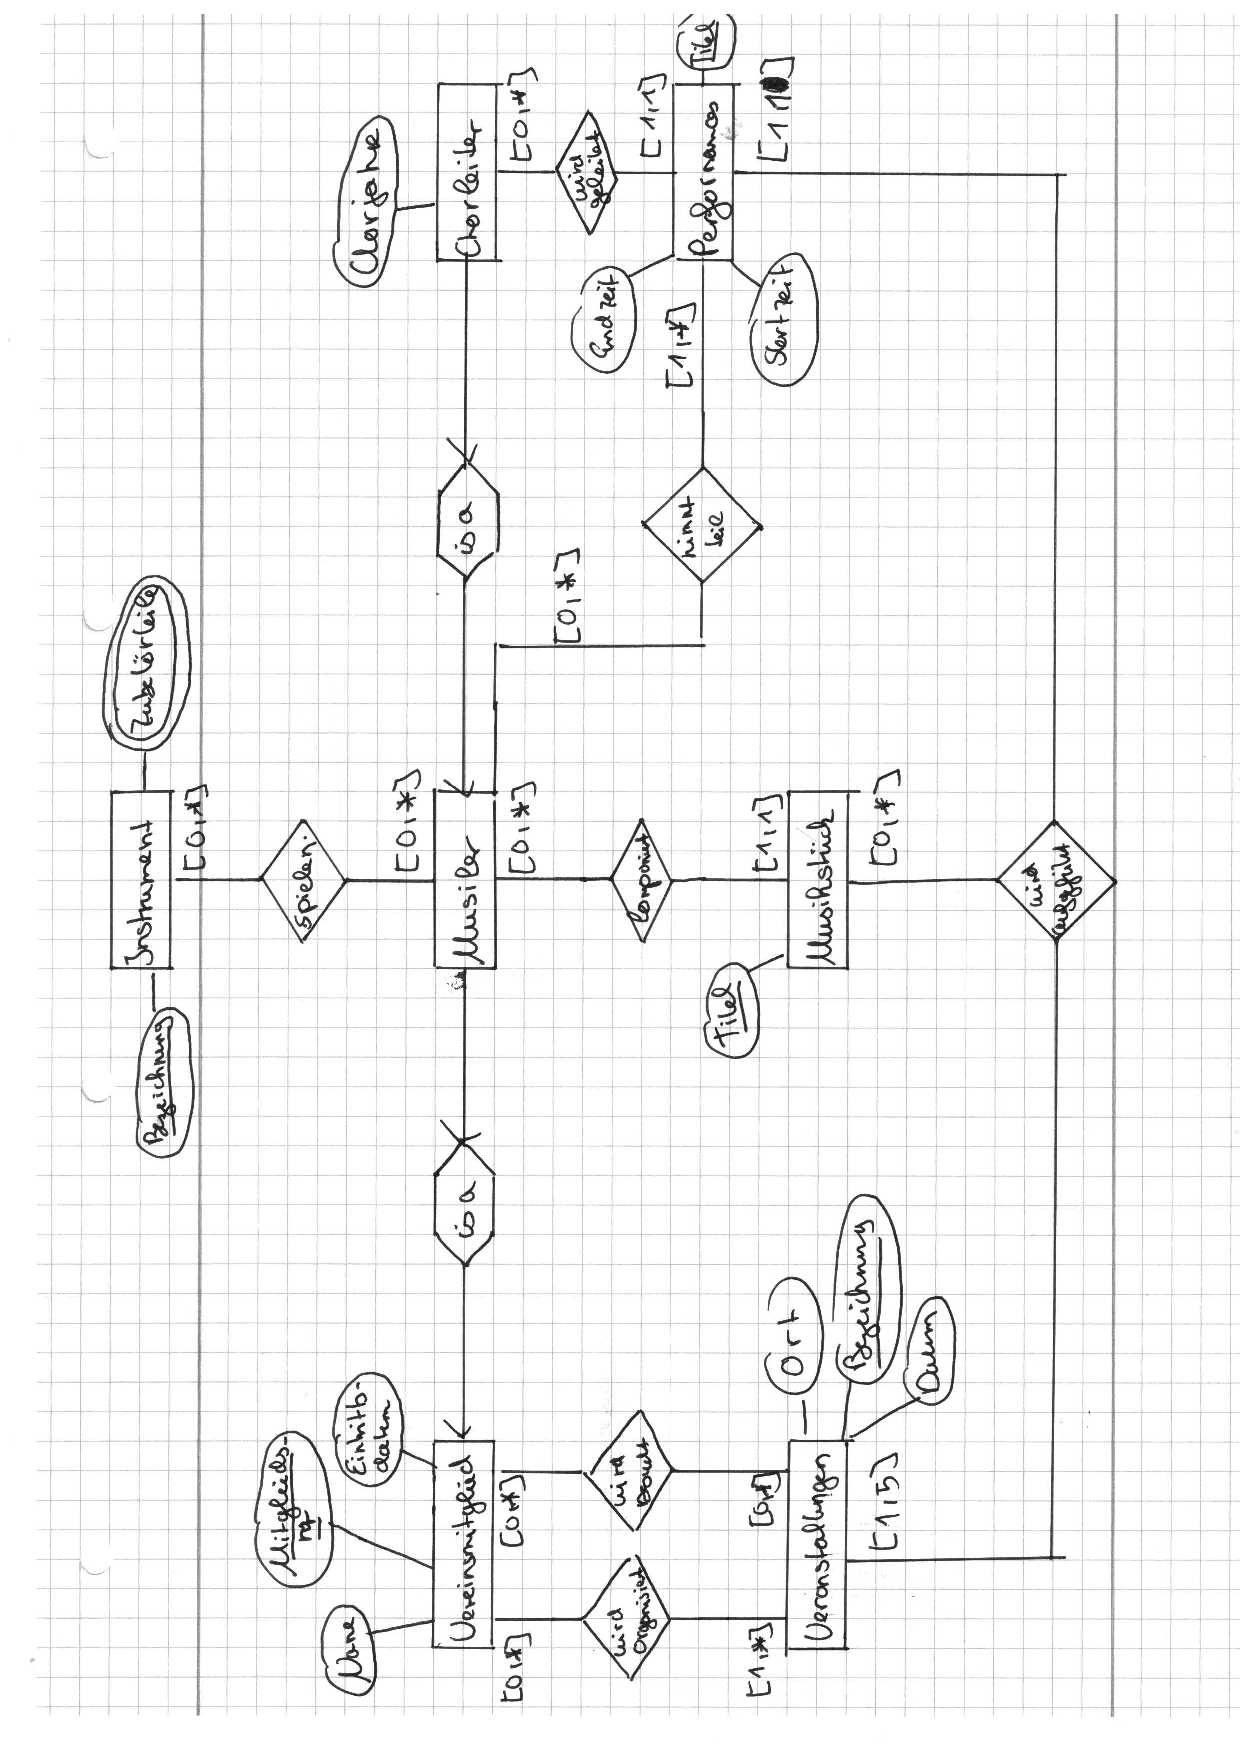
\includegraphics[height=10cm, angle=90]{diagramm}
\section{Abbildung eines ER-Diagramms auf das relationale Datenmodell}

\subsection{a)}
Modell(\underline{Datum, Name}, Grad) \\
Thema(\underline{Bez.}) \\
Zugeordnet(\underline{\dotuline{Bez. $\rightarrow$ Thema.Bez.}, \dotuline{Datum $\rightarrow$ Modell.Datum, Name $\rightarrow$ Modell.Name}}) \\
Set(\underline{SNr.}, Alter, \dotuline{Bez. $\rightarrow$ Thema.Bez.}) \\
Baustein(\underline{Form}, \dotuline{RGB $\rightarrow$ Farbe.RGB}) \\
Bild(\underline{\dotuline{Form $\rightarrow$ Baustein.Form}, Bild}) \\
Farbe(\underline{RGB}, CMYN) \\
Enth�lt(\underline{\dotuline{SNr. $\rightarrow$ Set.SNr.}, \dotuline{Form $\rightarrow$ Baustein.Form}, \dotuline{RGB $\rightarrow$ Farbe.RGB},}\\
\underline{ \dotuline{Datum $\rightarrow$ Modell.Datum, Name $\rightarrow$ Modell.Name}}, Teil-Anzahl) \\
Verkaufset(\underline{\dotuline{SNr. $\rightarrow$ Set.SNr}}, LPreis) \\
Werbeset(\underline{\dotuline{SNr. $\rightarrow$ Set.SNr.}}, Firma) \\

\subsection{b)}
Das Hausklassenmodell kann in dieser Relation nicht gut angewendet werden, da keine Informationen �ber die Vererbungen angegeben sind, bez�glich Set, Verkaufsset und Werbeset. Im Hausklassenmodell werden z.b. zum Verkaufsset die Attribute von Set mitangegeben, so dass wenn ein Set ein Verkaufsset ist, kein Set mehr ist.

\section{Relationale Algebra und SQL}
\subsection{a)}
$\pi$ $_{Titel}$($\sigma$ $_{Seitenzahl > 200 \wedge Erscheinungsjahr > 1950}$)
\begin{itemize}
\item Hundert Jahre Einsamkeit
\item Requiem f�r einen Traum
\item Der Talisman
\end{itemize}

$\pi$ $_{Vorname, Nachname}$(($\sigma$ $_{Buch.Titel = Der Talisman}$(schreibt)) $\bowtie$ Person)
\begin{itemize}
\item Stephen, King
\item Peter, Straub
\end{itemize}

$\pi$ $_{Vorname, Nachname}$($\sigma$ $_{Begutachtet.Buch = Person.Lieblingsbuch}$(Person $\bowtie$ Begutachtet))
\begin{itemize}
\item Leo, Tolstoi
\item Fjodor, Dostojewski
\item Gabriel, Garc�a M�rquez
\end{itemize}

\subsection{b)}
Es werden alle Informationen �ber die B�cher, die nicht begutachtet worden sind, ausgegeben.
\begin{itemize}
\item Schall und Wahn, 1929, 304, Diogenes
\item Der Talisman, 1984, 714, Heyne
\end{itemize}

Vorname und Nachname der Personen, die sowohl Lektor als auch Autor sind.
\begin{itemize}
\item Leo, Tolstoi
\item Fjodor, Dostojewski
\item Albert, Camus
\item William, Faulkner
\item Stephen, King
\item Peter, Straub
\item Gabriel, Garc�a M�rquez
\end{itemize}

Vorname und Nachname der Personen, die sowohl Lektor als auch Autor sind.
\begin{itemize}
\item Leo, Tolstoi
\item Fjodor, Dostojewski
\item Albert, Camus
\item William, Faulkner
\item Stephen, King
\item Peter, Straub
\item Gabriel, Garc�a M�rquez
\end{itemize}

\subsection{c)}
SELECT DISTINCT Vorname, Nachname FROM Person INNER JOIN Schreibt
ON Person.PID=Schreibt.Autor,(SELECT * FROM Buch WHERE Seitenzahl > 500) WHERE Schreibt.Buch = Buch.Titel;
\begin{itemize}
\item Leo, Tolstoi
\item Fjodor, Dostojewsk
\item Stephen, King
\item Peter, Straub
\end{itemize}
SELECT Buch.Titel FROM Schreibt WHERE Schreibt.Autor = Begutachtet.Lektor
\begin{itemize}
\item Schuld und S�hne
\item Krieg und Frieden
\item Anna Karenina
\item Hundert Jahre Einsamkeit
\item Der Talisman
\item Schall und Wahn
\item Als ich im Sterben lag
\item Der Fremde
\end{itemize}
SELECT Vorname, Nachname FROM Person WHERE Person.PID NOT IN (SELECT Begutachtet.Lektor FROM Begutachtet)
\begin{itemize}
\item Hubert, Selby
\end{itemize}

\section{Algebraische Optimierung}


\end{document}
